\section{Software}

\subsection{Principe général}

Le logiciel pilote le scanner et transforme une série d'images du plan
laser déformé par l'objet en un modèle 3D exportable (STL ou OBJ),
conformément aux exigences \textbf{E6} (format de sortie) et \textbf{E13}
(traitement, filtrage, export) du cahier des charges.

Le traitement suit un pipeline linéaire à quatre étages :
\textbf{Acquisition} $\rightarrow$ \textbf{Traitement} $\rightarrow$
\textbf{Reconstruction} $\rightarrow$ \textbf{Export}. Une machine d'états
(FSM) orchestre les transitions et garantit la cohérence des signaux
utilisateur (LEDs, écran, interface web), en réponse à l'exigence
\textbf{E5} (retour visuel).

\subsection{Architecture logicielle}

L'architecture est modulaire : chaque responsabilité est isolée dans un
sous-paquet Python exposant une API stable. Cette séparation permet le
développement sans matériel (mock caméra/moteur/laser) et le remplacement
ciblé d'un étage sans impacter les autres.

\begin{figure}[H]
  \centering
  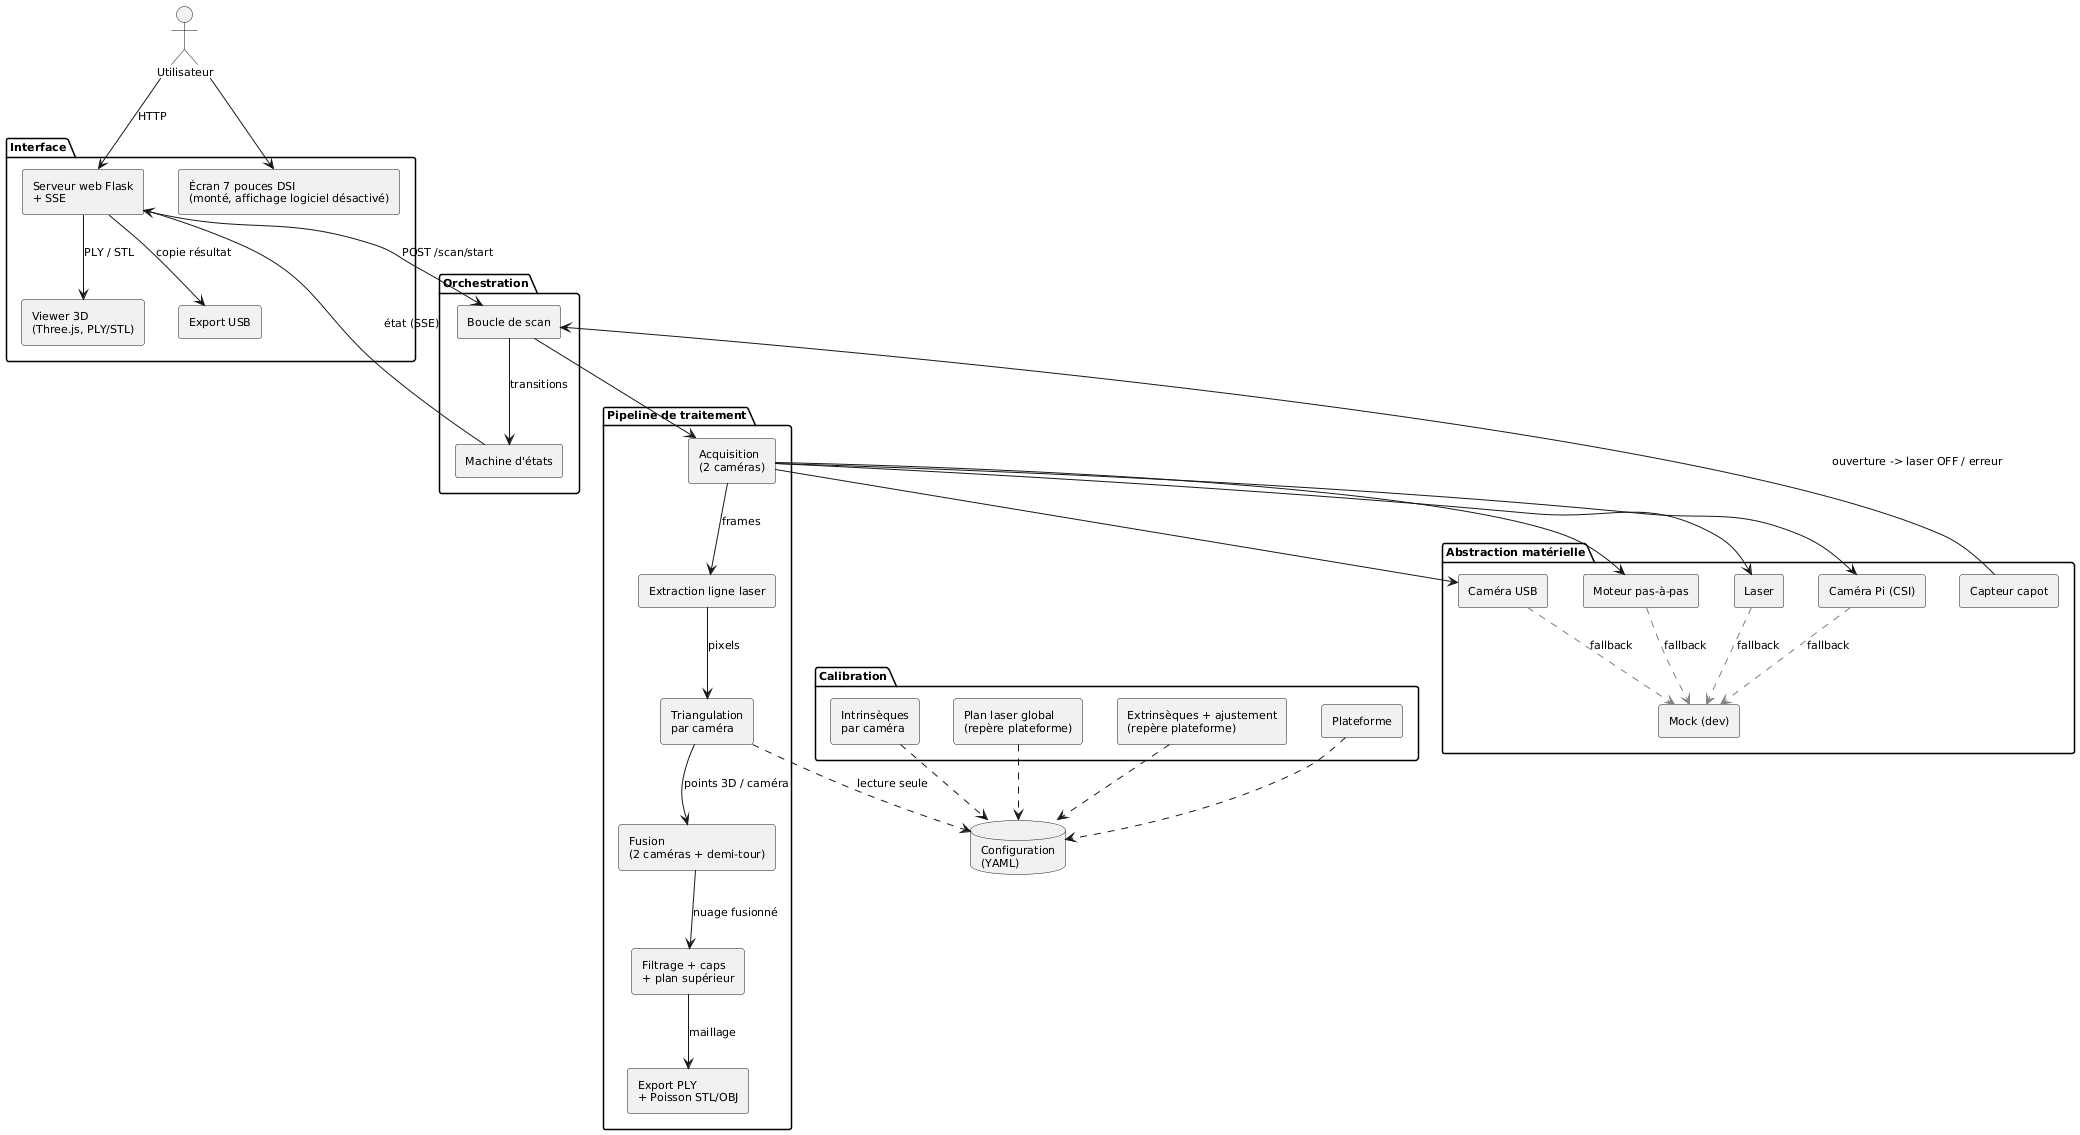
\includegraphics[width=\linewidth]{diagrams/architecture_composants.png}
  \caption{Architecture logicielle — vue des composants et flux de données.}
  \label{fig:archi-composants}
\end{figure}

\subsubsection{Modules}

\begin{table}[H]
  \centering
  \begin{tabular}{@{}p{3.5cm}p{10.5cm}@{}}
    \toprule
    \textbf{Module} & \textbf{Responsabilité} \\
    \midrule
    \texttt{hardware}       & Abstraction GPIO (moteur, laser, LEDs, caméra). Bascule automatique vers un \emph{mock} lorsque \texttt{gpiozero} est indisponible. \\
    \texttt{acquisition}    & Boucle capture : un pas moteur, allumage laser, capture image, extinction laser, sauvegarde. \\
    \texttt{processing}     & Extraction de la ligne laser (seuillage $G-R$, centroïde sous-pixel) et triangulation pixel $\rightarrow$ point 3D. \\
    \texttt{reconstruction} & Fusion des profils, filtrage d'\emph{outliers} par KDTree. \\
    \texttt{export}         & Génération STL / OBJ via \emph{convex hull} \texttt{trimesh}. \\
    \texttt{orchestration}  & Machine d'états et workflow de scan. \\
    \texttt{calibration}    & Calibration intrinsèque caméra (OpenCV) et plan laser. \\
    \texttt{interface}      & Serveur web Flask + SSE, affichage local TFT. \\
    \bottomrule
  \end{tabular}
  \caption{Modules logiciels et responsabilités.}
  \label{tab:modules}
\end{table}

\subsubsection{Flux de données}

La figure~\ref{fig:sequence-scan} détaille la séquence d'un cycle complet.
Pour un tour de plateau, 200 images sont acquises (pas de $1{,}8^\circ$),
chacune produisant un profil 2D, puis un nuage de points 3D par
triangulation avec le plan laser calibré.

\begin{figure}[H]
  \centering
  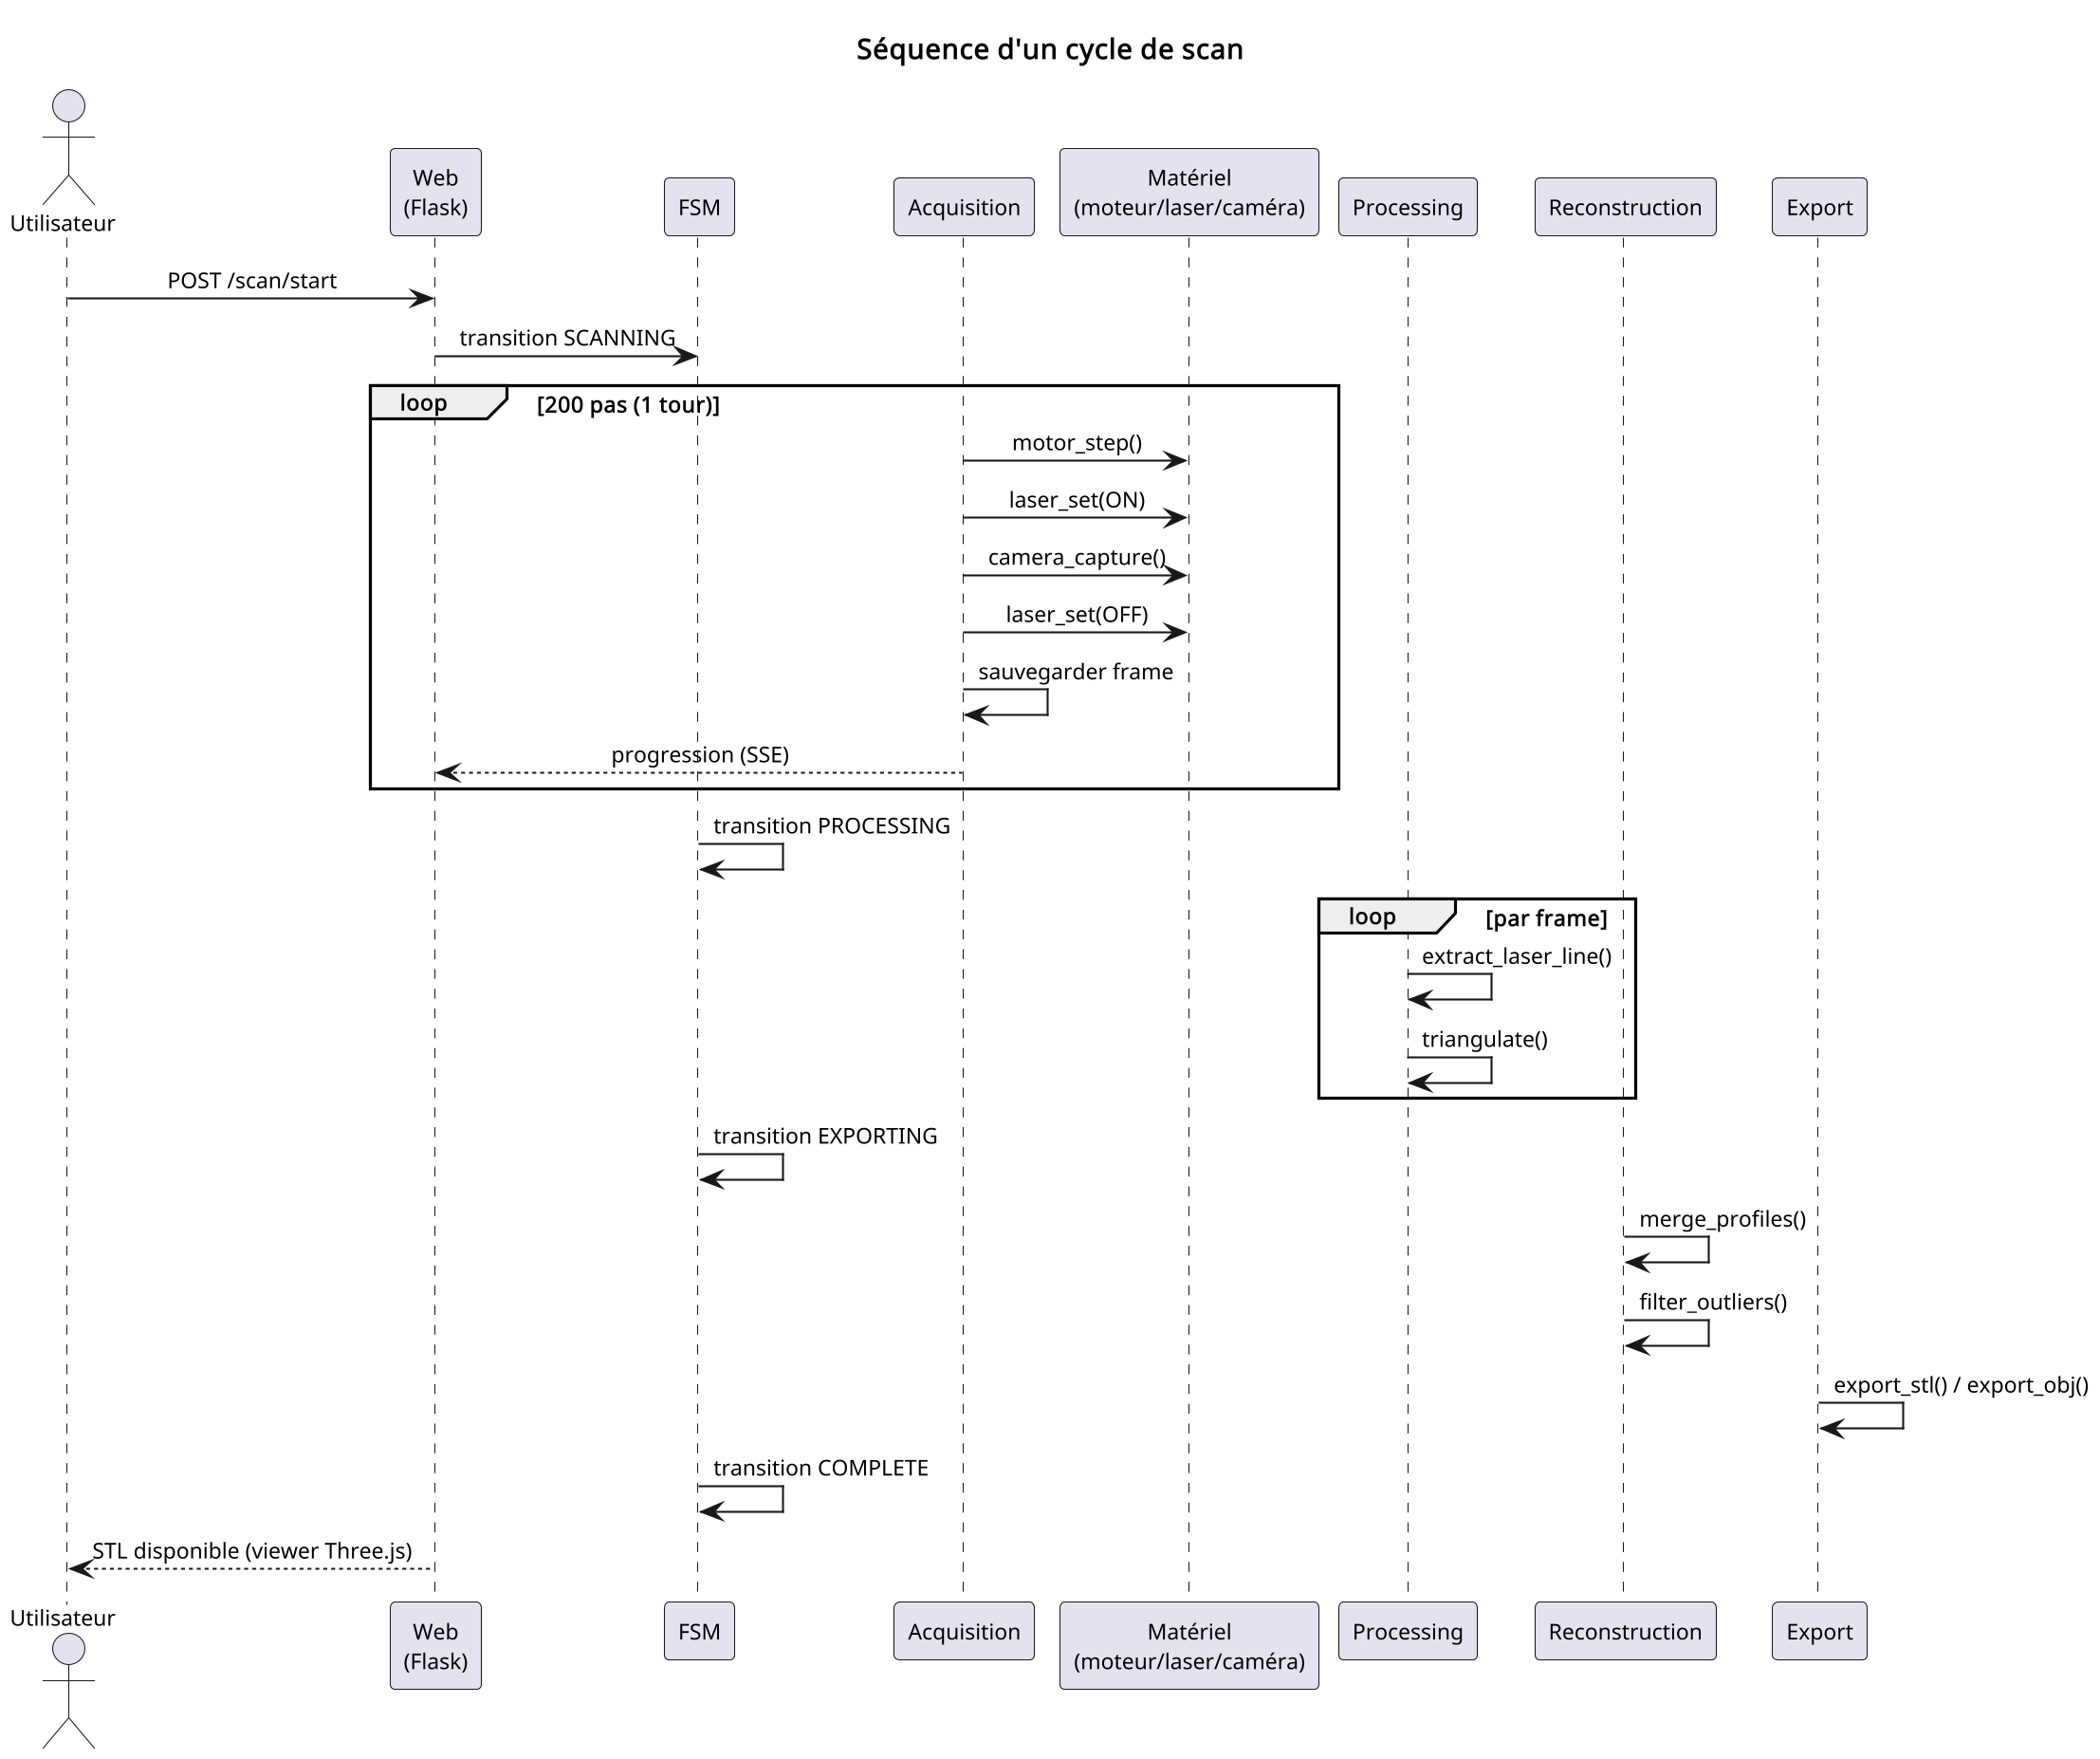
\includegraphics[width=0.95\linewidth]{diagrams/sequence_scan.png}
  \caption{Diagramme de séquence d'un cycle de scan.}
  \label{fig:sequence-scan}
\end{figure}

\subsection{Orchestration et machine d'états}

La FSM centralise les transitions légales et déclenche les effets de bord
associés (changement de LED, arrêt du laser en cas d'erreur). Les états
\texttt{IDLE}, \texttt{CALIBRATING}, \texttt{SCANNING}, \texttt{PROCESSING},
\texttt{EXPORTING}, \texttt{COMPLETE} et \texttt{ERROR} couvrent
l'ensemble du cycle de vie. Toute transition invalide lève une
exception plutôt qu'un état incohérent.

\begin{figure}[H]
  \centering
  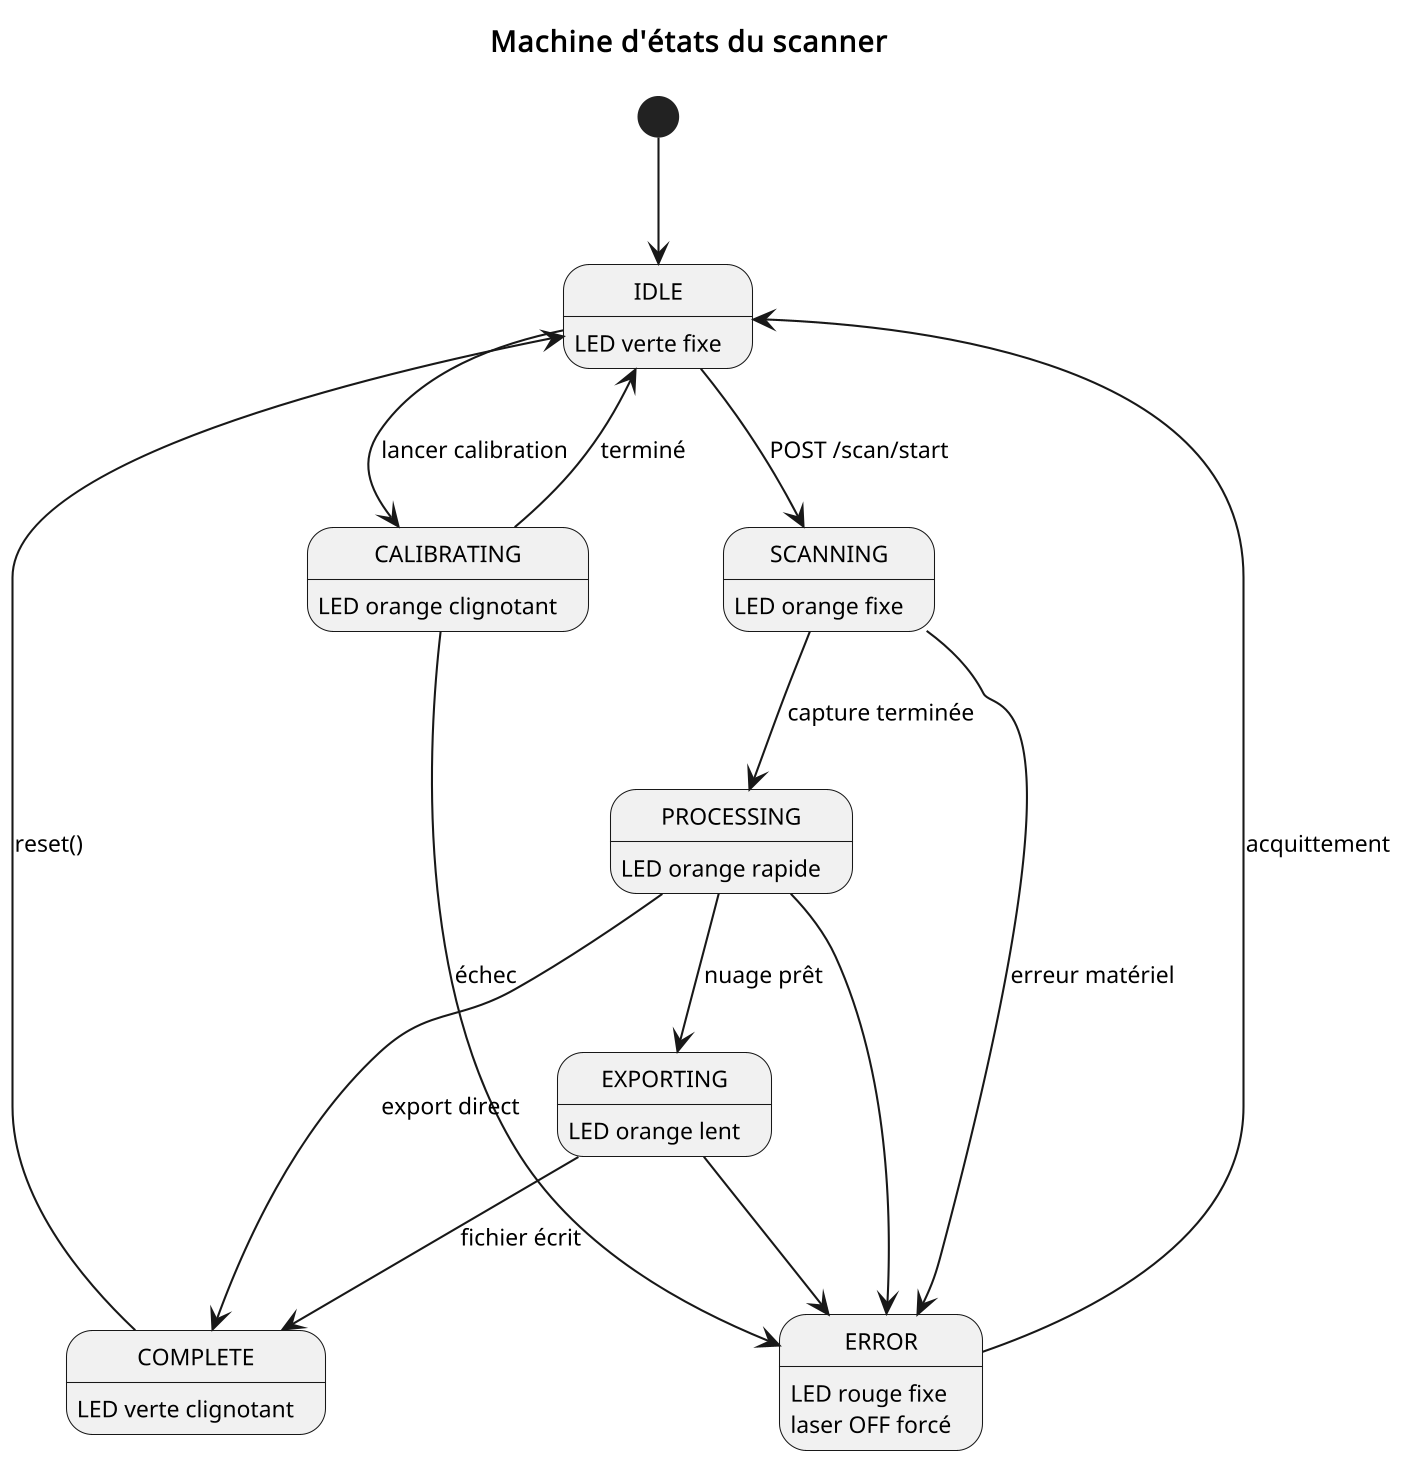
\includegraphics[width=0.85\linewidth]{diagrams/machine_etats.png}
  \caption{Machine d'états du scanner — transitions et signalisation LED.}
  \label{fig:fsm}
\end{figure}

\paragraph{Sécurité laser (exigence E19).}
Le laser est désactivé par défaut au démarrage. Un passage en
\texttt{ERROR} force sa coupure via un \emph{observer} de la FSM. Aucune
routine de calibration ne l'active sans confirmation. Un interrupteur de
porte (SW1, voir section électronique) complète la protection matérielle.

\subsection{Calibration}

Trois fichiers YAML, lus en lecture seule par le pipeline de scan,
stockent les paramètres calibrés :

\begin{itemize}
  \item \texttt{camera\_intrinsics.yaml} : matrice $3\times3$
        $(f_x, f_y, c_x, c_y)$ et coefficients de distorsion
        $(k_1, k_2, p_1, p_2, k_3)$, obtenus par damier + OpenCV.
  \item \texttt{laser\_plane.yaml} : équation du plan laser
        $[a, b, c, d]$ dans le repère caméra.
  \item \texttt{platform.yaml} : point de l'axe de rotation et nombre
        de pas par tour.
\end{itemize}

La règle d'immutabilité à l'exécution (le scan ne modifie jamais ces
fichiers) garantit la reproductibilité.

\subsection{Interface utilisateur}

L'interface web Flask (exigence \textbf{E10, E11}) expose les routes
nécessaires au lancement du scan, au suivi temps réel via Server-Sent
Events et au téléchargement du résultat. Un viewer Three.js charge
directement le STL binaire. Un afficheur TFT local reproduit l'état
courant pour un usage sans écran externe.

\subsection{Choix techniques}

\begin{table}[H]
  \centering
  \begin{tabular}{@{}p{4cm}p{4cm}p{6cm}@{}}
    \toprule
    \textbf{Besoin} & \textbf{Choix} & \textbf{Justification} \\
    \midrule
    Traitement d'image      & OpenCV          & Calibration caméra intégrée, léger sur Pi. \\
    Calcul numérique        & NumPy           & Standard scientifique Python. \\
    Filtrage de nuage       & SciPy KDTree    & Plus léger qu'Open3D sur Pi. \\
    Export maillé           & trimesh         & Support STL/OBJ sans dépendance GUI. \\
    GPIO                    & gpiozero        & API haut niveau, fallback \texttt{RPi.GPIO}. \\
    Interface web           & Flask + SSE     & Simple, SSE pour les mises à jour sans WebSocket. \\
    Viewer 3D               & Three.js        & Lecture native du STL binaire. \\
    Tests                   & pytest          & Standard, tous les GPIO mockés. \\
    \bottomrule
  \end{tabular}
  \caption{Bibliothèques et justifications.}
  \label{tab:choix-tech}
\end{table}

\subsection{Points ouverts}

\begin{itemize}
  \item Reconstruction concave (Poisson, \emph{alpha shape}) : actuellement
        \emph{convex hull}, suffisant pour un MVP mais limité pour les formes
        creuses. \emph{À compléter lors de la V2.}
  \item Export sur clé USB : stratégie de montage automatique à définir.
  \item Performances de bout en bout à mesurer pour respecter la cible
        de scan $<$ 10\,min (besoin B4 du CDC V2) et la précision
        \textbf{E24} ($\leq 2$\,mm d'erreur absolue, $\leq 1$\,mm de
        répétabilité). \emph{Mesures terrain à reporter.}
\end{itemize}
